\documentclass[a4paper,12pt,times,numbered,print,index]{Classes/PhDThesisPSnPDF}

\ifsetCustomMargin
  \RequirePackage[left=37mm,right=30mm,top=35mm,bottom=30mm]{geometry}
  \setFancyHdr % To apply fancy header after geometry package is loaded
\fi

\raggedbottom


\ifsetCustomFont
  
\fi

% ********************Captions and Hyperreferencing / URL **********************

\RequirePackage[labelsep=space,tableposition=top]{caption}
\renewcommand{\figurename}{Fig.} %to support older versions of captions.sty


% *************************** Graphics and figures *****************************

\usepackage{subcaption}

% ********************************** Tables ************************************
\usepackage{booktabs} % For professional looking tables
\usepackage{multirow}

% *********************************** SI Units *********************************
\usepackage{siunitx} % use this package module for SI units


% ******************************* Line Spacing *********************************

% ************************ Formatting / Footnote *******************************

% *****************************************************************************
% *************************** Bibliography  and References ********************

%\usepackage{cleveref} %Referencing without need to explicitly state fig /table

% Add `custombib' in the document class option to use this section
\ifuseCustomBib
   \RequirePackage[square, sort, numbers, authoryear]{natbib} % CustomBib

\fi

\renewcommand{\bibname}{References}


% ******************************************************************************
% ************************* User Defined Commands ******************************
% ******************************************************************************

% *********** To change the name of Table of Contents / LOF and LOT ************

% ********************** TOC depth and numbering depth *************************

\setcounter{secnumdepth}{2}
\setcounter{tocdepth}{2}


% ******************************* Nomenclature *********************************

% ********************************* Appendix ***********************************

% *********************** Configure Draft Mode **********************************

% ******************************** Todo Notes **********************************

% ************************ Thesis Information & Meta-data **********************
% Thesis title and author information, refernce file for biblatex
% ************************ Thesis Information & Meta-data **********************
\title{Prediction Markets for Machine Learning}
\subtitle{Master thesis in COMPUTER SCIENCE}
\author{Krzysztof Jerzy Geras}
\dept{Faculty of Mathematics, Informatics and Mechanics}
\university{University of Warsaw}
\crest{
\includegraphics[width=0.8\textwidth]{Fig/University_Warsaw}}
\degreetitle{Master of Computer Science}
\degreedate{September 2011} 
\subject{Machine Learning} \keywords{{Machine Learning} {Master Thesis} {Engineering} {University of Warsaw}}


% ***************************** Abstract Separate ******************************

\ifdefineAbstract
 \pagestyle{empty}
 
\fi

% ***************************** Chapter Mode ***********************************

\ifdefineChapter
 
\fi

% ******************************** Front Matter ********************************
\begin{document}

\frontmatter

\maketitle


% ******************************* Thesis Declaration ***************************

% ************************** Thesis Abstract *****************************
\begin{abstract}
The main topic of the thesis is prediction markets as a machine learning tool. The thesis gives
an overview of current state of the art in this research area, relates artificial prediction markets
to existing well-known model combination techniques and shows how they extend them.
It also develops techniques introduced in one of previously known frameworks, contains a
description of a first practical implementation of this framework and evaluates its performance
on both synthetic and real data sets from UCI machine learning repository. Finally, results
of this evaluation are utilised to understand strengths and weaknesses of this approach and
to suggest future directions in this research area.
\end{abstract}
\clearpage

% *********************** Adding TOC and List of Figures ***********************

\tableofcontents

\listoffigures

\listoftables

\printnomenclature

% ******************************** Main Matter *********************************
\mainmatter



%!TEX root = ../thesis.tex
%*******************************************************************************
%****************************** First Chapter **********************************
%*******************************************************************************
\chapter{Background}

% **************************** Define Graphics Path **************************
\graphicspath{{Chapter1/}}

\section{Supervised and unsupervised learning}

If an algorithm is given a set of inputs (also called features vectors) {x1, x2, . . . , xn} and a set
of corresponding outputs (also called labels) {y1, y2, . . . , xn} and the goal of the algorithm is
to learn to produce the correct output given a new input, this is a supervised learning task.
A supervised learning task is called classification if the outputs are discrete or regression if
the outputs are continuous.
If an algorithm is only given a set of inputs {x1, x2, . . . , xn} and no outputs, this is an
unsupervised learning task. Unsupervised learning can be thought of as finding patterns in
the data above and beyond what would be considered pure unstructured noise. Two most
common examples of unsupervised learning are clustering and dimensionality reduction.
Inputs can be vectors of different types of objects, integer numbers, real numbers, strings
or more complex objects. Outputs take values each representing a unique state. For example,
an algorithm may be given a number of vectors representing numerically external features
of a person, such as height, weight, shoe size etc., and corresponding outputs that take one
value from the set {male, female}.

\section{Classification}

Classification is a particular supervised learning task. The objective of a classification algorithm
is, given a set of inputs X, that come from a space F
L, and corresponding outputs Y,
that belong to one of K classes, to learn a function that can predict an output for unseen input.
Usually a good measure of performance of a classifier is misclassification rate.
Sometimes it’s more convenient to use accuracy, which is equal to 1 - M.
If an algorithm outputs a probability distribution over classes and not just predicted class,
then it learns a function. In that case, a good complementary measure can be log-likelihood.
This may be a good measure in some circumstances as it does not asses how often the classifier
was right, instead assessing how much probability mass it put on the correct class.
Practical classification algorithms include: support vector machines, logistic regression,
neural networks, k nearest neighbours, decision trees and Naive Bayes. Ensemble methods
(section 1.4) build more complex models using these. Please see [HasTibFri09] for a comprehensive
overview.
It is important to understand that function h not only has to describe the training data
(X, Y) but also has to be able to generalize to unseen instances. If a classifier has a very
low misclassification rate on training data but high misclassification rate on test data, it
is said to overfit to the training data. That means that the classifier models the noise in
the training data and not the true underlying pattern that is of our interest. Overfitting
occurs primarily when the model has too many parameters given the amount of training data
available. Therefore, it is very often reasonable to favour simpler models to more complex
ones. Figure 1.1 shows an example of this phenomenon.
Predicting classifier’s performance on unseen data, should never be done on the training
data, overfitting is one the reasons. It is typically the best approach, to partition the data into
three sets: training set - to train the classifier, validation set - to tune classifier’s parameters
and test set - to predict performance on new instances.

\section{Clustering}

Clustering is an unsupervised learning task. The objective is to divide a set of objects,
represented by inputs {x1, x2, ..., xn}, into a set of disjoint clusters {{x1,1, x1,2, ..., x1,n1
},{x2,1, x2,2, ..., x2,n2}, ..., {x3,1, x3,2, ..., x3,n3}}, that contain objects similar to each other
in some sense. Typically, similarity between two objects is defined by Euclidean distance or Manhattan distance.
For a comprehensive overview on clustering algorithms please refer to [Fun01].

\section{Ensemble methods}

Ensemble methods use multiple models to combine them into one stronger model. Experience
shows that it is common for individual algorithms to be outperformed by combinations of models and heterogeneous combinations are of special interest ([BelKor07]). As mentioned
by [Die00] there are essentially three reasons why ensembles of models perform better than
individual models: statistical, computational and representational.

\begin{figure}
\centering    
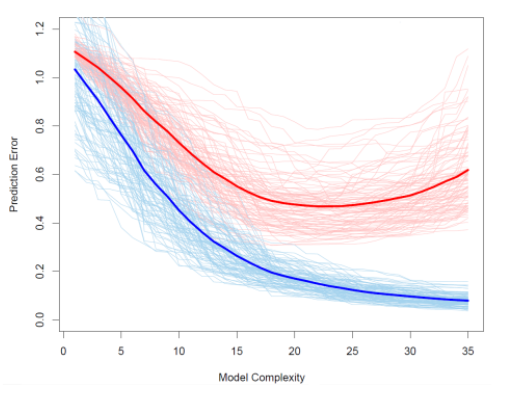
\includegraphics[width=1.0\textwidth]{1}
\caption[1]{First figure}
\label{fig:1}
\end{figure}

\begin{figure}
\centering    
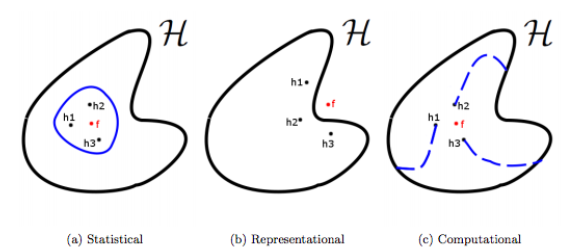
\includegraphics[width=1.0\textwidth]{2}
\caption[2]{Second figure}
\label{fig:2}
\end{figure}

\begin{enumerate}
  \item Statistical. One way to look at a learning algorithm is to view it as searching a hypothesis
space H to find the best one. Without enough data the algorithm may find a few
different hypotheses in H that give the same accuracy on the training (or validation)
data. By constructing an ensemble, the algorithm can find a point that is, in a certain
sense, an average of the members of the ensemble and thus reduces a risk of choosing
the wrong classifier.
  \item Representational. In many cases the true function f cannot be represented within hypothesis
space H. By combining classifiers into an ensemble it may be possible to expand a
set of representable functions. Even though some algorithms, like neural networks (that
actually are universal approximators as shown in [Hor91]), can, in theory, express a lot
of functions, it is important to bear in mind that due to the finite amount of training
data, they will effectively explore a finite number of hypotheses and will stop when the
model fits the training data well enough.
  \item Computational. Even when there is enough data, an algorithm performing local search for
the best hypothesis may get stuck in local optima. That is the case for neural networks
for example. Therefore, starting from different points and combining obtained models
in an ensemble may lead to a model that is closer to the true hypothesis.
The most widely used ensemble methods are Random Forest ([Bre01]) and AdaBoost
([Sch03]).
\end{enumerate}

\subsection{Random Forest}

Decision trees
A decision tree partitions the feature space into rectangular regions and assigns a class to
every region. The process of partitioning the space is performed in such a way that the
choice of the variable that will be responsible for current split is done by greedily picking a
variable that gives the highest information gain. Decision trees are conceptually very simple
yet accurate. Algorithm 1 gives a precise description on how to build a decision tree.

\subsection{AdaBoost}

Boosting, and also more specifically the AdaBoost algorithm, is based on the observation that
finding a single, very accurate prediction rule is much harder than finding many rough rules.
AdaBoost builds multiple weak classifiers, feeding a classification algorithm with a different
distribution of training examples each round. At the end of that process, the algorithm
combines those weak learners, that have to be only slightly better than random, into one
strong classifier.
The two important questions in this approach are how to change the distribution of
training examples and how to combine classifiers. AdaBoost answers the first question by
putting more weight on those examples that are harder to learn and combines classifiers by
plain weighted majority voting, where the weights are chosen according to equations (1.6)
and (1.7).


% ********************************** Back Matter *******************************

% ********************************** Bibliography ******************************
\begin{spacing}{0.9}

\bibliographystyle{apalike}
\cleardoublepage
\bibliography{References_references} % Path to your References.bib file

\end{spacing}

% ********************************** Appendices ********************************

\begin{appendices} % Using appendices environment for more functunality

\end{appendices}

% *************************************** Index ********************************
\printthesisindex % If index is present

\end{document}
